%% LyX 2.3.6.2 created this file.  For more info, see http://www.lyx.org/.
%% Do not edit unless you really know what you are doing.
\documentclass{beamer}
\usepackage[latin9]{inputenc}
\setcounter{secnumdepth}{3}
\setcounter{tocdepth}{3}
\usepackage{booktabs}
\usepackage{amstext}
\usepackage{graphicx}

\makeatletter

%%%%%%%%%%%%%%%%%%%%%%%%%%%%%% LyX specific LaTeX commands.
%% Because html converters don't know tabularnewline
\providecommand{\tabularnewline}{\\}

%%%%%%%%%%%%%%%%%%%%%%%%%%%%%% Textclass specific LaTeX commands.
% this default might be overridden by plain title style
\newcommand\makebeamertitle{\frame{\maketitle}}%
% (ERT) argument for the TOC
\AtBeginDocument{%
  \let\origtableofcontents=\tableofcontents
  \def\tableofcontents{\@ifnextchar[{\origtableofcontents}{\gobbletableofcontents}}
  \def\gobbletableofcontents#1{\origtableofcontents}
}

%%%%%%%%%%%%%%%%%%%%%%%%%%%%%% User specified LaTeX commands.
\usetheme{Madrid}
\usepackage{listings}
\usepackage{xcolor}
\usepackage{tabularx}
\usepackage{fancyvrb}



\title{Understanding BERT's [CLS] Token for Long Texts}
\subtitle{From Short Sentences to Document-Level Representation}
\author{Qingfeng Liu}
\institute{Hosei University}
\date{\today}

\makeatother

\begin{document}
\begin{frame}
\titlepage 
\end{frame}
% Slide 2: Core Concept

\begin{frame}{Core Concept}

\frametitle{The {[}CLS{]} Token's Role}
\begin{itemize}
\item Regardless of input length, BERT always outputs: 
\begin{itemize}
\item A \textbf{fixed-length} 768-dim vector for `{[}CLS{]}` 
\item Preserves semantic information through: 
\begin{itemize}
\item Self-attention mechanisms 
\item Pretraining objectives (MLM + NSP) 
\end{itemize}
\end{itemize}
\end{itemize}
\begin{block}{Key Property}
\textbf{Input length agnostic}: Same output dimension whether input
is 1 word or 1000 words (with processing) 
\end{block}
\end{frame}
% Slide 3: Short vs Long Text Processing

\begin{frame}{Short vs Long Text Processing}

\frametitle{Comparison}

\begin{table}
\centering %
\begin{tabular}{lcc}
\toprule 
\textbf{Feature}  & \textbf{Short Text}  & \textbf{Long Text} \tabularnewline
\midrule 
Input length  & $<$ 512 tokens  & $\geq$ 512 tokens \tabularnewline
Processing  & Direct encoding  & Requires segmentation \tabularnewline
{{[}CLS{]}} quality  & High precision  & Potential information loss \tabularnewline
Example  & \texttt{"Cat catches mouse"}  & Research papers \tabularnewline
\bottomrule
\end{tabular}
\end{table}
\end{frame}
% Slide 4-5: Long Text Handling Methods

\begin{frame}{BERT - Code}
\centering 

\begin{figure}

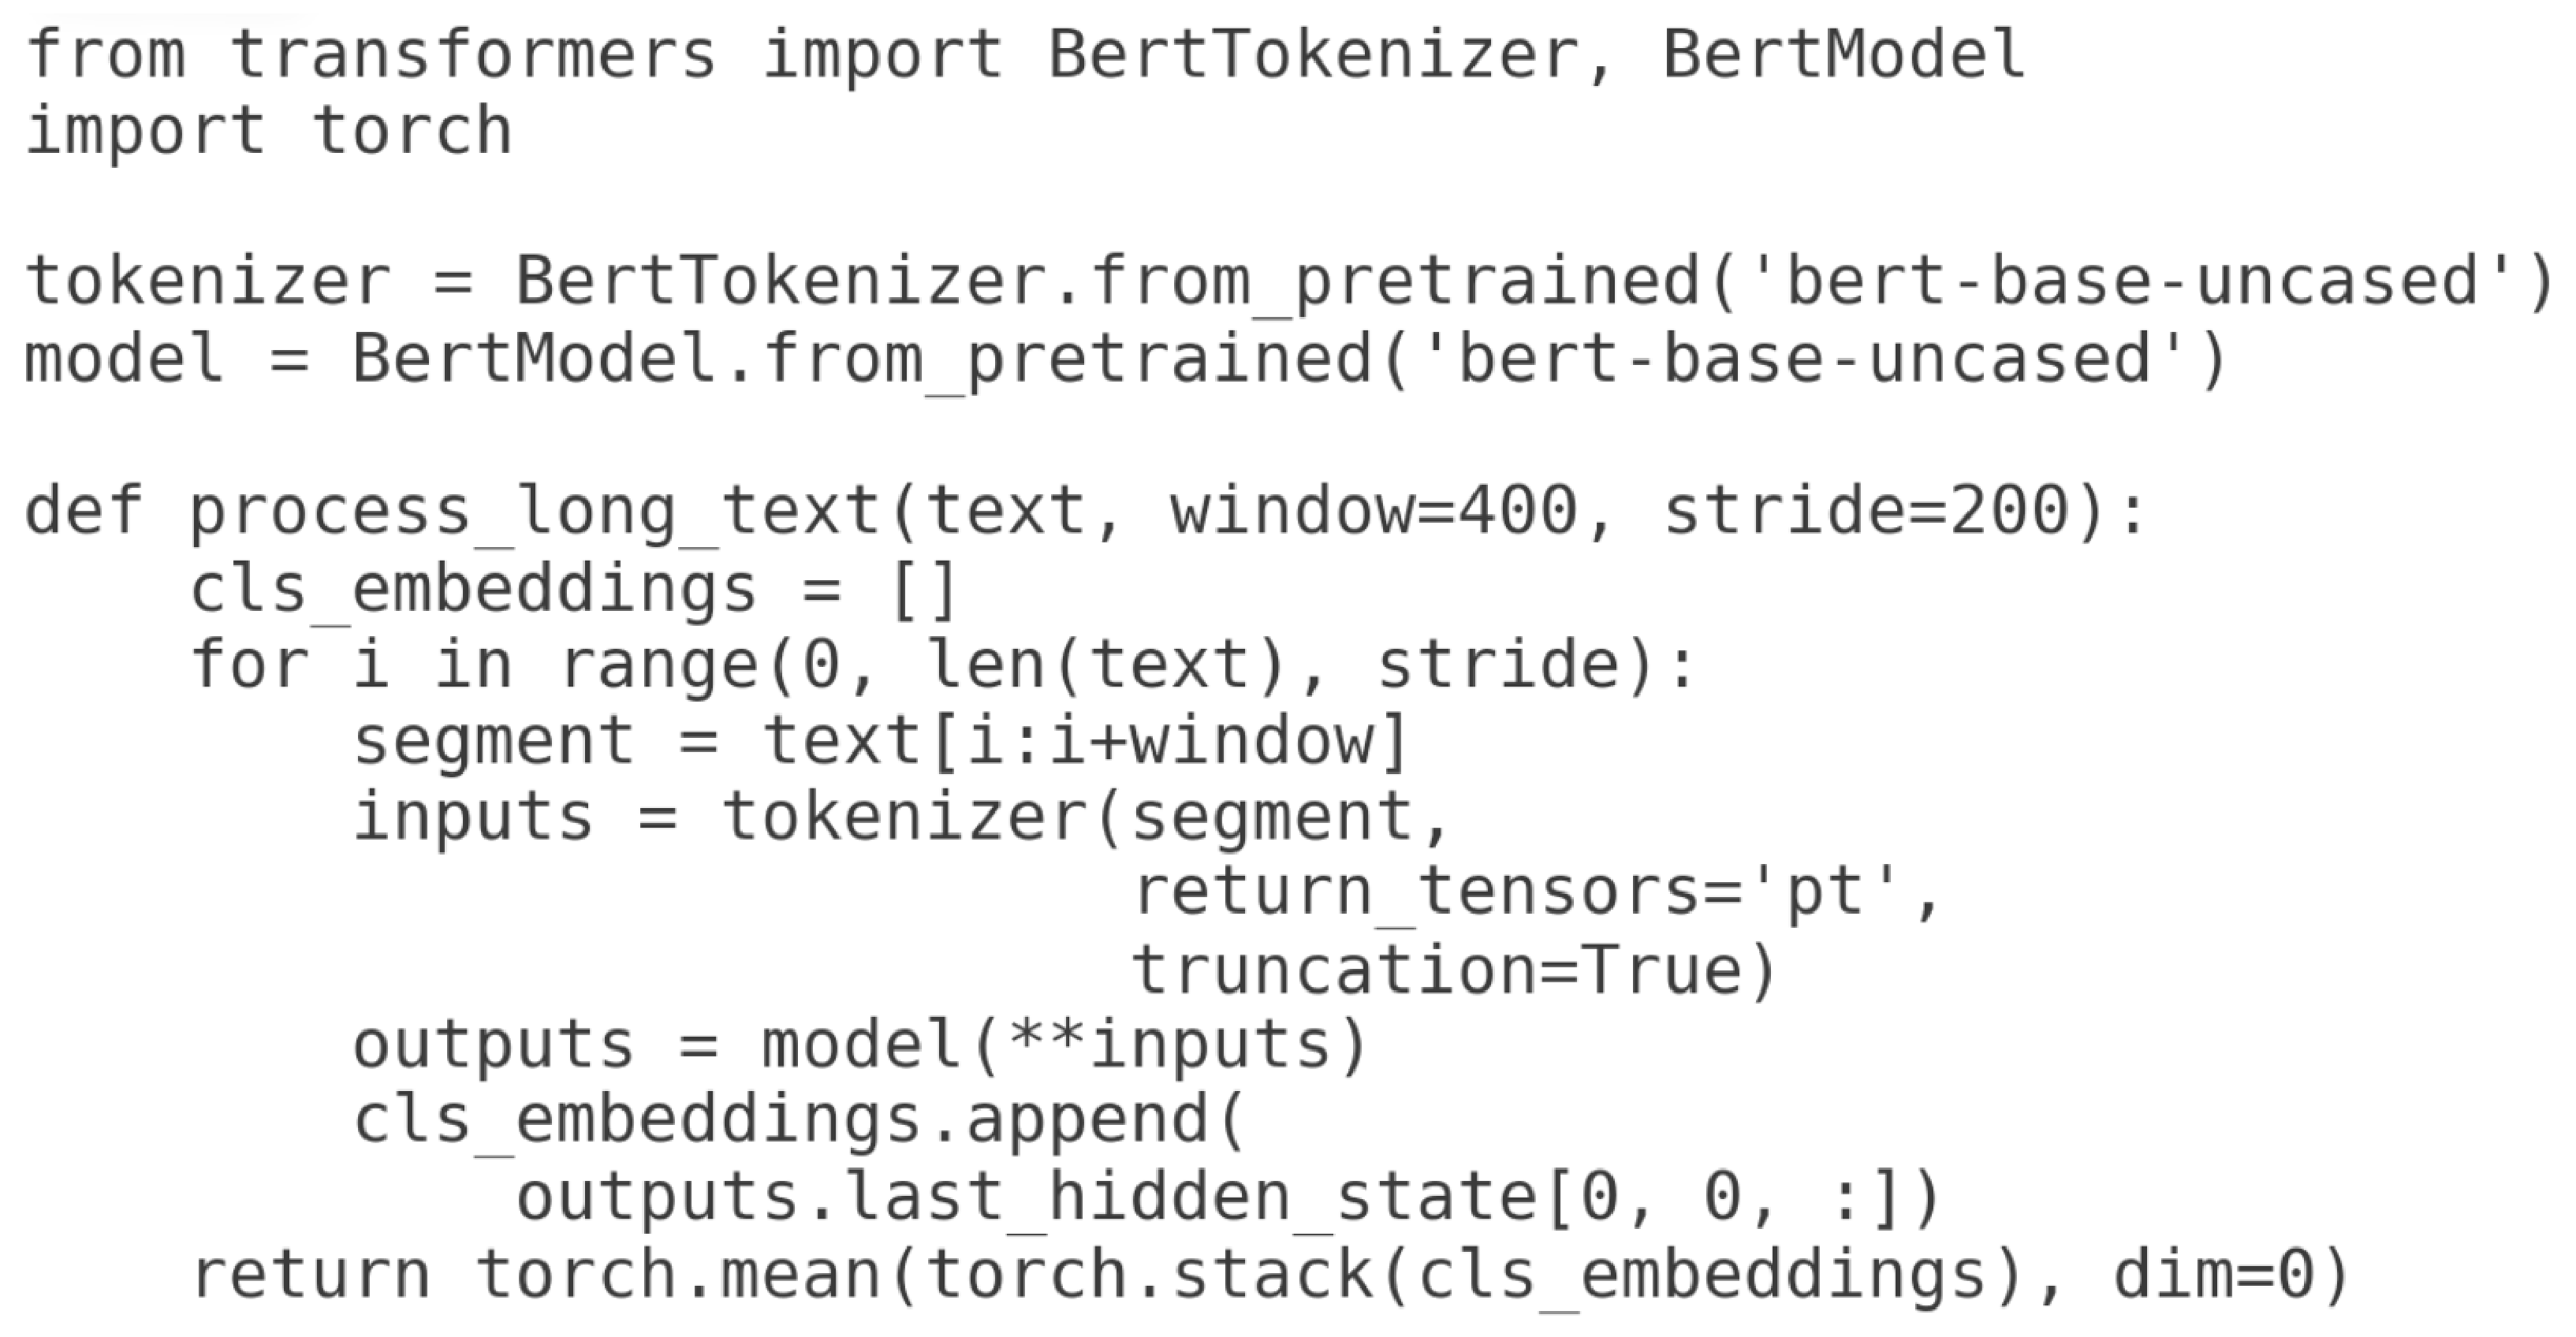
\includegraphics[width=11cm]{../Figures/pasted1}

\end{figure}
\end{frame}
% Slide 7: Mathematical Representation

\begin{frame}{Mathematical Formulation}

\frametitle{Aggregating Multiple {[}CLS{]} Vectors}

For document $D$ divided into $n$ segments: 
\[
\text{FinalEmbedding}=\frac{1}{n}\sum_{i=1}^{n}\text{[CLS]}_{i}
\]

Where: 
\begin{itemize}
\item $\text{[CLS]}_{i}$ is the vector from the $i^{th}$ segment 
\item Averaging maintains the 768-dimension output 
\end{itemize}
\begin{example}
For 2000-token document with 500-token windows: 
\begin{itemize}
\item 4 segments $\rightarrow$ 4 {[}CLS{]} vectors 
\item Final embedding = mean of 4 vectors 
\end{itemize}
\end{example}

\end{frame}
% Slide 8: Why This Works

\begin{frame}{Why This Approach Works}

\frametitle{Theoretical Foundation}
\begin{itemize}
\item \textbf{Attention Propagation}: 
\begin{itemize}
\item Each window's `{[}CLS{]}` attends to local context 
\item Global semantics emerge through aggregation 
\end{itemize}
\item \textbf{Pretraining Alignment}: 
\begin{itemize}
\item NSP task trains BERT to combine segment information 
\item MLM ensures local context understanding 
\end{itemize}
\item \textbf{Dimensionality Preservation}: 
\begin{itemize}
\item Each `{[}CLS{]}` is 768-dim $\rightarrow$ mean is 768-dim 
\item Compatible with downstream models 
\end{itemize}
\end{itemize}
\end{frame}
% Slide 9: Comparison Table

\begin{frame}{Method Comparison}

\frametitle{Performance Characteristics}

\begin{table}[h]
\centering {\small{}}%
\begin{tabular}{lccc}
\toprule 
\textbf{\small{}Method}{\small{} } & \textbf{\small{}Info Retention}{\small{} } & \textbf{\small{}Speed}{\small{} } & \textbf{\small{}Use Case}{\small{} }\tabularnewline
\midrule 
{\small{}Truncation } & {\small{}Low } & {\small{}Fast } & {\small{}Real-time apps }\tabularnewline
{\small{}Sliding Window } & {\small{}Medium } & {\small{}Medium } & {\small{}Document classification }\tabularnewline
{\small{}Hierarchical } & {\small{}High } & {\small{}Slow } & {\small{}Legal/medical analysis }\tabularnewline
\bottomrule
\end{tabular}
\end{table}
\begin{itemize}
\item Trade-off between completeness and efficiency 
\item Window overlap (25-50\%) improves continuity 
\end{itemize}
\end{frame}
% Slide 10: Recommendations

\begin{frame}{Best Practices}

\frametitle{Implementation Tips}
\begin{block}{For Standard Documents (500-2000 tokens)}
\begin{itemize}
\item Use sliding window with: 
\begin{itemize}
\item Window size: 400-500 tokens 
\item Stride: 200-300 tokens 
\end{itemize}
\item Mean pooling for aggregation 
\end{itemize}
\end{block}
\end{frame}
%
\begin{block}{For Very Long Texts (10k+ tokens)}
\begin{itemize}
\item Consider: 
\begin{itemize}
\item Extractive summarization first 
\begin{itemize}
\item Domain-specific models (e.g., Longformer) 
\end{itemize}
\end{itemize}
\end{itemize}
\begin{alertblock}{Warning}
Avoid simple truncation for mission-critical applications 
\end{alertblock}
\end{block}
% Slide 11: Complete Pipeline

\begin{frame}{Complete Processing Pipeline}

\frametitle{End-to-End Flow}
\begin{enumerate}
\item \textbf{Preprocessing}: 
\begin{itemize}
\item Clean text 
\item Handle special characters 
\end{itemize}
\item \textbf{Segmentation}: 
\begin{itemize}
\item Split into valid BERT windows 
\item Add overlap if needed 
\end{itemize}
\item \textbf{Embedding Generation}: 
\begin{itemize}
\item Process each segment 
\item Extract `{[}CLS{]}` vectors 
\end{itemize}
\item \textbf{Aggregation}: 
\begin{itemize}
\item Mean/max pooling 
\item Optional dimensionality reduction 
\end{itemize}
\end{enumerate}
\end{frame}
% Slide 12: Conclusion

\begin{frame}{Conclusion}

\frametitle{Key Takeaways}
\begin{itemize}
\item \textbf{Single-vector output}: BERT always provides 768-dim `{[}CLS{]}`
regardless of input length 
\item \textbf{Long document handling} requires: 
\begin{itemize}
\item Segmentation strategy 
\item Careful aggregation 
\end{itemize}
\item \textbf{Sliding window} offers best balance for most applications 
\end{itemize}
\begin{block}{Final Note}
The `{[}CLS{]}` token serves as BERT's universal compression mechanism,
but intelligent preprocessing is crucial for long texts. 
\end{block}
\end{frame}

\end{document}
